\documentclass[conference]{IEEEtran}
\usepackage{amsmath,amssymb,amsfonts}
\usepackage{graphicx}
\usepackage{booktabs}
\usepackage{array}
\usepackage{url}
\usepackage[hidelinks]{hyperref}
\usepackage{tikz}
\usetikzlibrary{shapes.geometric, arrows.meta, positioning}

\begin{document}

\title{Secure Multi-QR File Storage and Transmission Using Encrypted Fragmentation and Controlled Reconstruction}

\author{\IEEEauthorblockN{N. Deepesh}
\IEEEauthorblockA{\textit{Department of Computer Science and Engineering} \\
\textit{Amrita Vishwa Vidyapeetham}, Amaravati, India}}

\maketitle

\begin{abstract}
QR codes are widely consumed for short web links and payment strings, though their use as a multi-symbol transport for arbitrary binary files receives far less attention in practical system design. When a whole file is forced into one QR image, symbol density rises sharply and ordinary scanners start failing. This paper investigates an end-to-end workflow for splitting, distributing, and rebuilding files across multiple QR codes. In our implemented baseline, the sender program takes an input file, compresses the byte stream with \texttt{zlib}, cuts the output into 700-byte slices, assigns single-digit identifiers alongside one extra decoy payload, and outputs shuffled PNG images. On the other side, a Flask web interface checks the uploaded QR payloads and the user-entered sequence before concatenating the slices and comparing the final SHA-256 hash against the sender's original digest. Tested locally on Windows 11 under Python 3.13.12, the prototype handles up to eight genuine slices and one decoy, passing all 16 unit tests in 3.952 seconds as well as a browser-based binary reconstruction check on \texttt{random\_test.bin}. Still, the current build leaves payload bytes unencrypted and holds transfer state only in volatile process memory. To close these gaps, we propose an extended security design that combines authenticated X25519 key agreement, HKDF key derivation, AES-256-GCM encryption, a verified transfer manifest, persistent fragment storage, and short-lived retrieval tokens. Two operating modes are defined: direct byte embedding inside QR symbols for small files, and opaque token lookup for larger transfers. Because the cryptographic and storage layers remain at the design stage, we separate the tested baseline evidence from the six-month implementation and evaluation plan required prior to final deployment.
\end{abstract}

\begin{IEEEkeywords}
QR code, file fragmentation, secure file transfer, AES-GCM, X25519, HKDF, decoy payload, token-based retrieval, SHA-256.
\end{IEEEkeywords}

\section{Introduction}
When you scan a normal QR code with a phone camera, the payload is almost always a short URL, a text snippet, or a payment identifier. The underlying specification can represent raw binary data as well, yet putting an entire file into a single symbol runs into practical trouble right away. Either the file size exceeds what one QR symbol can hold, or the module grid becomes so dense that screen and camera decoding turns unreliable. How much data fits into a symbol depends on its version number, encoding mode, and Reed-Solomon error-correction level \cite{iso18004}, \cite{denso}. Splitting the file across a small batch of QR codes avoids that density bottleneck and lets us study how multi-part optical transfers can be reassembled under strict ordering rules.

Our project started with a straightforward implementation question: if we divide a compressed file across several QR images and slip a decoy symbol into the batch, how reliably can a web application enforce ordered reconstruction? In the working prototype, the sender uploads a file, records its SHA-256 digest, compresses the raw bytes with \texttt{zlib}, and slices the compressed stream into 700-byte chunks. Each genuine slice gets a unique single-digit ID from 1 to 9 using Python's \texttt{secrets} module. One additional decoy QR code is generated with matching byte length, and the image list is shuffled before display. To recover the file, the receiver uploads all the PNG images to our Flask interface and enters the genuine ID sequence. The server validates the JSON metadata inside each symbol, checks the submitted sequence against the active transfer record in memory, joins the genuine chunks, inflates the stream, and checks whether the resulting SHA-256 digest matches the sender's hash.

While this baseline confirms that the multi-QR reconstruction path works, its actual security exposure has to be stated plainly. Base64 only turns binary bytes into ASCII text, and \texttt{zlib} only removes statistical redundancy. If someone obtains the QR images, they can decode the JSON fields and inflate the byte slices directly without ever touching our Flask sequence check. Furthermore, the SHA-256 hash stored inside the QR metadata is unsigned, which means an attacker who modifies both the chunk bytes and the digest field can produce a self-consistent forgery \cite{fips180}.

For that reason, this paper treats the existing Flask application as a baseline testbed and sets out an extended architecture that links multi-QR delivery with encrypted fragment storage. In the proposed system, the sender compresses, encrypts, and slices the file before binding every fragment to an authenticated manifest. Small transfers can still place encrypted bytes straight into the QR symbols, whereas larger transfers store the ciphertext chunks on a server and put short-lived lookup tokens into the QR codes instead. Our specific focus is on how these standard building blocks fit together into a single verifiable workflow and how their failure modes should be tested.

\subsection{Problem and Objectives}
Dividing a file among several QR symbols creates problems that do not arise in a normal single-file upload. Chunks from different transfers may be mixed, a QR symbol may be missing or duplicated, and a user may attempt to retrieve stored fragments in the wrong order. The design therefore has five objectives: (1) retain direct-payload QR delivery for small files; (2) add opaque-token retrieval for larger transfers, where fragments are stored separately from the QR symbols; (3) protect file contents in transit and at rest through authenticated key agreement and AES-256-GCM encryption; (4) bind every fragment to an authenticated manifest and an explicit receiver-authorization policy; and (5) define a repeatable evaluation covering functional errors, cryptographic tampering, token replay, performance, and decoy detection.

\section{Related Work and Technical Background}
ISO/IEC 18004 specifies the physical layout, encoding modes, and error-correction rules used by QR Code symbols \cite{iso18004}. DENSO WAVE provides reference tables showing how byte capacity changes across symbol versions 1 through 40 \cite{denso}. These references describe individual symbols. They do not define how an application should associate several QR images with one original file or verify that the fragments have been assembled in the correct order.

Splitting data into pieces is also discussed in the context of Shamir's threshold secret sharing \cite{shamir}. In that scheme, any $k$ out of $n$ shares can reconstruct the secret, while fewer than $k$ shares reveal no information about it. The approach used in our prototype is different: it divides a compressed byte stream into consecutive ranges, and every genuine range must be present and restored in its original order before decompression can succeed. Our lossless compression pipeline uses \texttt{zlib} and DEFLATE, as specified in RFC 1950 and RFC 1951 \cite{rfc1950}, \cite{rfc1951}. When encryption is added, compression must take place first because encrypted data has high entropy and is not expected to compress further. End-to-end byte verification uses SHA-256, specified in NIST FIPS 180-4 \cite{fips180}.

The extended design uses established cryptographic and web-security standards. AES-GCM, specified in NIST SP 800-38D, provides authenticated encryption and integrity protection for ciphertext and associated authenticated data (AAD) \cite{sp80038d}. A nonce must not be reused with the same key, and the receiver must verify the authentication tag before accepting or releasing the decrypted plaintext. Shared-secret establishment uses X25519 elliptic-curve Diffie--Hellman \cite{rfc7748}, together with HKDF for key derivation \cite{rfc5869}. Raw X25519 does not authenticate the identity of the other party, so public keys must be verified through certificates, digital signatures, or an out-of-band fingerprint check to prevent man-in-the-middle substitution. File-upload and storage handling also follow the layered validation practices described by OWASP \cite{owasp}.

\section{Baseline System and Threat Model}
\subsection{Implemented Workflow}
In the current Python implementation, the sender uploads a file $F$, computes its digest $H = \mathrm{SHA256}(F)$, and compresses the file into a byte stream $C = \mathrm{zlib}(F)$. The chunk size is fixed at $m = 700\text{ bytes}$, so the number of genuine chunks is $n = \lceil |C|/m \rceil$, with $1 \le n \le 8$. The encoder then creates one random decoy byte sequence with the same length as the first genuine chunk. This gives $N = n + 1$ payloads, or at most nine QR symbols. Single-digit identifiers from 1 to $N$ are assigned using Python's \texttt{secrets} module. The PNG images are shuffled, while the sender interface displays the ordered sequence $S$ of genuine identifiers. The Flask process stores both $S$ and the decoy identifier $d$ in an active-transfer dictionary.

On the receiver page, the user uploads the QR images in any order and enters the sequence. The parser accepts spaces, commas, hyphens, or semicolons between digits. The server decodes each PNG using \texttt{zxing-cpp}, with an OpenCV grayscale-and-thresholding fallback. It checks that the JSON payloads belong to the same transfer UUID and contain the expected metadata, then compares the submitted sequence with the transfer state stored on the server. If the sequence matches $S$ and excludes $d$, the server concatenates the genuine chunks, decompresses the stream with a 100 MiB output limit, and checks whether the resulting SHA-256 digest matches $H$. If the decoy identifier is included or the submitted order is incorrect, the application returns harmless placeholder content through the dummy-file generator while preserving the original filename.

\subsection{Capacity and Current Limits}
The baseline supports at most eight genuine chunks, each with a maximum size of 700 bytes. The compressed stream $C$ is therefore limited to $8 \times 700 = 5{,}600\text{ bytes}$. The QR payload is larger than the raw chunk because the binary data is converted to Base64 before it is placed in the JSON structure. For example, 700 bytes become 936 Base64 characters, before adding fields such as \texttt{version}, \texttt{transfer\_id}, \texttt{filename}, \texttt{total\_qrs}, \texttt{sha256}, \texttt{compression}, and \texttt{qr\_id}. The \texttt{qrcode} library encodes the complete JSON string using error-correction level M. As a result, whether an input file fits depends on its compressed size and the space required for the encoded metadata. Plain-text files larger than 5,600 bytes may still fit if compression reduces them sufficiently. Pre-compressed ZIP archives, JPEG images, and high-entropy binary files usually shrink very little, so they may be rejected when the compressed stream requires more than eight chunks. Flask's separate 10 MB request limit only restricts the size of an HTTP upload; it does not increase the QR payload capacity.

The prototype also has clear security and deployment limits. Payload bytes are Base64-encoded, not encrypted, and the sender's identity is not cryptographically authenticated. The expected sequence and decoy identifier are kept in the memory of a single Flask process, so a server restart clears the active transfer records. The current implementation is therefore a local functional testbed for multi-QR reconstruction, not a hardened multi-user storage service.

\subsection{Threat Model}
In designing the extended architecture, we consider an adversary who can capture QR codes during transmission, inspect unencrypted JSON fields, monitor network traffic, upload malformed or duplicate symbols, combine fragments from separate transfers, reorder chunk sequences, or guess and replay lookup tokens. We assume that the adversary cannot break standard cryptographic primitives (AES-256-GCM, X25519, and SHA-256) or compromise the operating system of the sender, authorized receiver, or storage server. Observable traffic metadata, such as the number of QR symbols in a batch or approximate chunk sizes, is not hidden by encryption. When a decoy reference is triggered, the system records the event for review. However, this event alone is not definitive proof of an attack because an authorized user may also enter a digit incorrectly.

\begin{figure*}[t]
\centering
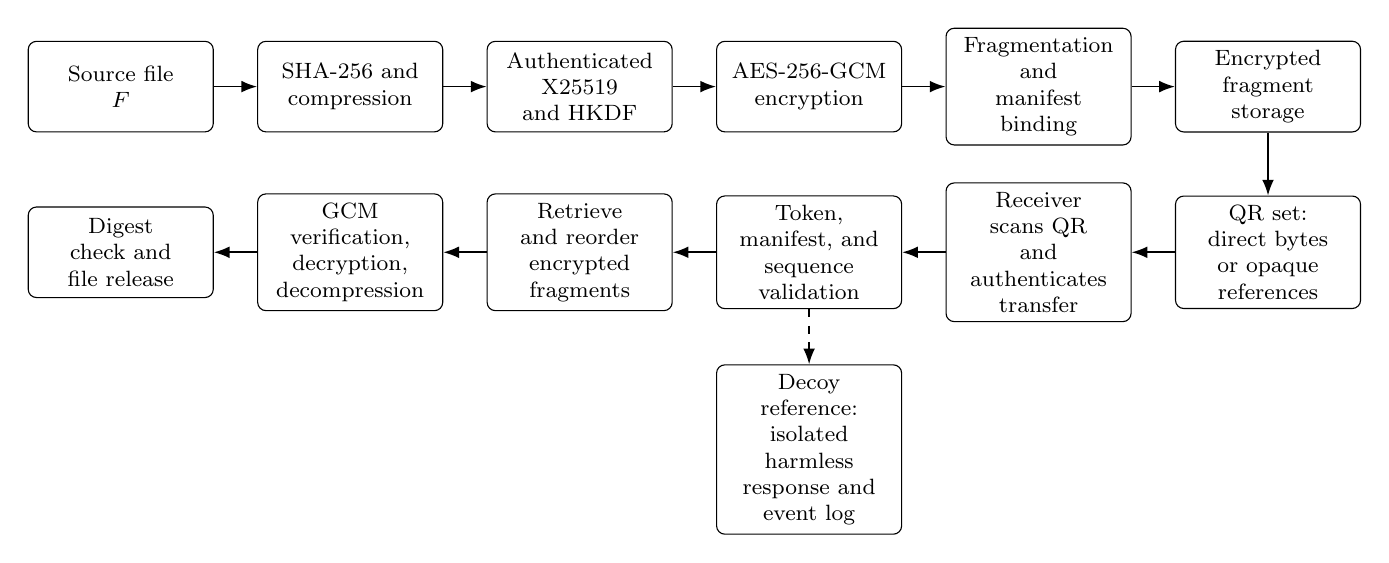
\begin{tikzpicture}[
    node distance=0.55cm and 0.55cm,
    box/.style={rectangle, draw, rounded corners=3pt, align=center, minimum width=2.35cm, minimum height=1.15cm, font=\footnotesize},
    arrow/.style={-{Latex[length=2mm, width=1.5mm]}, semithick}
]
% Row 1
\node[box] (f) {Source file\\$F$};
\node[box, right=of f] (sha) {SHA-256 and\\compression};
\node[box, right=of sha] (x25519) {Authenticated\\X25519\\and HKDF};
\node[box, right=of x25519] (aes) {AES-256-GCM\\encryption};
\node[box, right=of aes] (frag) {Fragmentation\\and\\manifest\\binding};
\node[box, right=of frag] (store) {Encrypted\\fragment\\storage};

% Row 2
\node[box, below=0.8cm of store] (qrset) {QR set:\\direct bytes\\or opaque\\references};
\node[box, left=of qrset] (scan) {Receiver\\scans QR\\and\\authenticates\\transfer};
\node[box, left=of scan] (val) {Token,\\manifest, and\\sequence\\validation};
\node[box, left=of val] (ret) {Retrieve\\and reorder\\encrypted\\fragments};
\node[box, left=of ret] (gcm) {GCM\\verification,\\decryption,\\decompression};
\node[box, left=of gcm] (dig) {Digest\\check and\\file release};

% Decoy box
\node[box, below=0.7cm of val] (decoy) {Decoy\\reference:\\isolated\\harmless\\response and\\event log};

% Arrows
\draw[arrow] (f) -- (sha);
\draw[arrow] (sha) -- (x25519);
\draw[arrow] (x25519) -- (aes);
\draw[arrow] (aes) -- (frag);
\draw[arrow] (frag) -- (store);
\draw[arrow] (store) -- (qrset);
\draw[arrow] (qrset) -- (scan);
\draw[arrow] (scan) -- (val);
\draw[arrow] (val) -- (ret);
\draw[arrow] (ret) -- (gcm);
\draw[arrow] (gcm) -- (dig);
\draw[arrow, dashed] (val) -- (decoy);
\end{tikzpicture}
\caption{Integrated sender-to-receiver architecture. Direct QR payloads are intended for small transfers; retrieval references point to encrypted fragments in controlled storage.}
\label{fig:arch}
\end{figure*}

\section{Integrated Secure Architecture}
To address the limits of the baseline, the extended architecture divides the work across four entities: a sender client, a receiver client, an application server that manages transfer state and access policies, and an encrypted fragment store. Fig.~\ref{fig:arch} shows the complete data path. A basic rule of this layout is that decryption keys are never combined with storage lookup tokens. Scanning a QR symbol provides either ciphertext bytes or a reference to retrieve them, but never the key material needed to decrypt them.

\subsection{Sender Pipeline and Key Establishment}
The sender pipeline starts by calculating the SHA-256 digest of the original file $F$ and then compressing it with \texttt{zlib}. The sender and receiver then perform an authenticated X25519 key exchange. Because an unauthenticated Diffie--Hellman exchange can be intercepted by an active man-in-the-middle, peer public keys must be verified using certificates, digital signatures, or a trusted out-of-band fingerprint check \cite{rfc7748}, \cite{rfc5869}. HKDF uses the resulting shared secret to derive two separate keys for each transfer: one for AES-256-GCM encryption and another for manifest authentication. Ephemeral private keys are generated using a cryptographically secure random source and discarded from active application state after key derivation.

The compressed byte stream is then encrypted using AES-256-GCM with a fresh nonce. Essential manifest fields are passed as AAD so that any header tampering invalidates the authentication tag. The resulting ciphertext and GCM tag are divided into sequential fragments. At the receiver, the complete ciphertext is reassembled and its GCM authentication tag is checked before any plaintext is released, decompressed, or written. If a later version uses per-fragment streaming decryption for very large files, each fragment will require its own unique nonce and AAD that binds the transfer UUID, fragment index, and total fragment count.

\subsection{Manifest, Fragment Storage, and QR Modes}
Before the QR codes are distributed, the sender creates a versioned transfer manifest. It contains the protocol version, transfer UUID, cipher suite, GCM nonce, ciphertext length, fragment count and indices, compression format, expected SHA-256 digest of the plaintext, and authorized receiver context. The manifest is protected using the HKDF-derived authentication key or a sender digital signature. Fragments are stored using both the transfer UUID and fragment index, so fragments from two different transfers cannot be combined.

Two delivery modes are used depending on the transfer size. In direct-payload mode, the QR symbols carry the encrypted fragment bytes and header fields directly. This keeps small transfers self-contained without requiring a live storage service, although total capacity is still limited by QR version, symbol density, and fragment count. In retrieval-link mode, the encrypted fragments are written to persistent storage, and each QR symbol carries only a high-entropy opaque lookup reference. This moves the size bottleneck from QR capacity to server storage and network bandwidth, but it requires service availability, token expiry checks, and authenticated HTTP retrieval.

Lookup references in retrieval mode act only as access tokens, not as encryption keys. Each token is generated using a CSPRNG and scoped to a single transfer and fragment index. It is given a short time-to-live (TTL), protected against guessing through rate limiting, and checked for receiver authorization on every request. Raw token strings must also be excluded from server logs, analytics headers, and browser Referer fields. The storage backend must also apply explicit retention and cleanup rules.

\subsection{Decoy Handling}
If a decoy QR code has a different JSON structure or token length from genuine symbols, an observer can identify it easily. In the extended design, decoy payloads use the same outer schema, field names, and identifier format as real fragment references. Submitting a decoy token sends the request to an isolated handler that returns harmless placeholder bytes and records minimal event data, including a pseudonymous token hash, timestamp, and response outcome. This handler is kept separate from real fragment storage and does not ask for user credentials. The design does not claim that decoys are indistinguishable under every possible side channel. Instead, their effectiveness will be measured against a clearly defined inspection procedure.

\subsection{Transfer Validation and Retrieval Lifecycle}
After the authenticated X25519 exchange, HKDF generates the encryption key $K_e$ and the manifest authentication key $K_m$:
\begin{equation}
(K_e, K_m) = \mathrm{HKDF}(Z, \mathrm{salt}, \mathrm{context}).
\end{equation}
The compressed stream $C$ is encrypted with key $K_e$ using AES-GCM and a unique nonce $N$: $X = \mathrm{AES\text{-}GCM.Enc}(K_e, N, C, A)$, where $A$ contains the authenticated transfer context. The output $X$, which includes the ciphertext and authentication tag, is divided into $k$ sequential fragments $X_1, \dots, X_k$. The accompanying manifest is then authenticated with a MAC under $K_m$ or signed by the sender.

In retrieval mode, each stored fragment $X_i$ is assigned a random, high-entropy token. The database stores only a hashed token verifier, together with the transfer UUID, fragment index, expiry timestamp, and consumption state. A lookup succeeds only when the token verifier matches, the token has not expired or been revoked or used, and the authenticated receiver is permitted by the manifest policy. Each transfer moves through defined lifecycle states (\texttt{created}, \texttt{distributed}, \texttt{active}, \texttt{completed}, and \texttt{expired}/\texttt{revoked}). Garbage-collection jobs wait for active downloads to finish or time out before deleting the stored chunks.

At the receiver, the client verifies the manifest MAC or signature and checks that all $k$ fragments belong to the same transfer UUID and have the complete set of indices $1 \dots k$. It then reorders the fragments, verifies the AES-GCM authentication tag, decompresses the stream within the 100 MiB output limit, and compares the resulting file's SHA-256 hash with the manifest digest $H_F$:
\begin{equation}
\begin{split}
\mathrm{Accept} &= \mathrm{ValidManifest} \land \mathrm{Complete}(X_1, \dots, X_k) \\
&\quad \land \mathrm{ValidTag} \land (\mathrm{SHA256}(F') = H_F).
\end{split}
\end{equation}
If any check in (2) fails, the original file is withheld. Incorrect sequences or decoy selections are sent to the rate-limited dummy-response path.

\begin{table}[t]
\caption{Implemented Baseline and Extended Design Status}
\label{tab:status}
\centering
\begin{tabular}{>{\raggedright\arraybackslash}p{0.34\columnwidth} >{\raggedright\arraybackslash}p{0.56\columnwidth}}
\toprule
\textbf{Component} & \textbf{Status and Boundary} \\
\midrule
Compression, chunking, and QR generation & Implemented with \texttt{zlib}, 700-byte chunks, up to eight genuine chunks and one decoy. \\
\addlinespace[3pt]
Sequence validation and reconstruction & Implemented; expected sequence and decoy ID are retained in server memory. \\
\addlinespace[3pt]
Integrity check & SHA-256 comparison tested; digest is not a sender-authentication mechanism. \\
\addlinespace[3pt]
AES-GCM and authenticated X25519 & Extended design; not part of the current baseline. \\
\addlinespace[3pt]
Persistent retrieval and token policy & Extended design; requires storage, expiry, authorization, and replay controls. \\
\addlinespace[3pt]
Decoy monitoring & Design requirement; isolated event handling and effectiveness remain to be tested. \\
\bottomrule
\end{tabular}
\end{table}

\begin{table}[t]
\caption{Required Evaluation Before Final Submission}
\label{tab:eval}
\centering
\begin{tabular}{>{\raggedright\arraybackslash}p{0.24\columnwidth} >{\raggedright\arraybackslash}p{0.66\columnwidth}}
\toprule
\textbf{Area} & \textbf{Test and Evidence to Report} \\
\midrule
Functional & Correct reconstruction; missing, duplicate, reordered, or mixed-transfer fragments; unsupported or malformed payloads. \\
\addlinespace[3pt]
Cryptographic & Modified ciphertext, invalid GCM tag, wrong key, nonce-policy checks, and substituted or unauthenticated peer keys. \\
\addlinespace[3pt]
Retrieval & Expired, replayed, revoked, guessed, and unauthorized tokens; access after restart; rate-limit behaviour. \\
\addlinespace[3pt]
Reliability & QR scan failures, interrupted retrieval, storage outage, fragment loss, backup restoration, and cleanup. \\
\addlinespace[3pt]
Performance & Sender/receiver time, QR generation and scan time, retrieval latency, storage/network overhead, and concurrent receivers. \\
\addlinespace[3pt]
Deception & Decoy-versus-genuine distinguishability under a stated attacker view, plus false-positive and event-log checks. \\
\bottomrule
\end{tabular}
\end{table}

\section{Security and Correctness Analysis}
\textbf{Confidentiality:} When the X25519-derived keys are properly authenticated and an AES-GCM nonce is never reused with the same key, AES-256-GCM prevents an eavesdropper or storage administrator from reading the compressed file bytes. Traffic metadata, including the number of symbols, request timing, and approximate fragment size, remains observable on the network. Application code must also make sure that temporary buffers or error logs never write raw plaintext.

\textbf{Integrity and Authenticity:} Any change to the ciphertext or AAD causes AES-GCM tag verification to fail before decompression. Authenticating the manifest prevents an attacker from changing the transfer UUID, altering the fragment count, or replacing the expected SHA-256 digest. Keeping the SHA-256 check after decompression provides an additional end-to-end check that the reconstructed file matches the original file.

\textbf{Availability:} All fragments must be available for sequential reconstruction. If one QR code is damaged beyond level-M error correction or the storage server loses a fragment, the file cannot be recovered. Operational availability therefore depends on storage replication, backups, and retry handling rather than cryptography.

\textbf{Sequence and Decoy Controls:} Checking the submitted digit sequence enforces the intended workflow, while rate limiting helps prevent automated attempts to guess digit permutations. Decoy logs may alert operators to probing, but user mistakes can also trigger them; therefore, they are indicators, not proof of malicious activity.

\section{Implementation and Evaluation}
The basic prototype was developed in Python and tested locally on Windows 11 in a Python 3.13.12 virtual environment. Flask serves the web interface through separate Sender and Receiver routes. QR images are generated using \texttt{qrcode} with Pillow, while decoding uses \texttt{zxing-cpp} with an OpenCV fallback. A 16-case \texttt{unittest} suite checks valid reconstruction, incorrect sequence order, decoy substitution or addition, missing or duplicate QR symbols, duplicate sequence digits, malformed Base64 strings, mixed transfer UUIDs, unsafe filenames and path traversal, digest mismatches, and dummy PDF/file generation. In the recorded local run, all 16 unit tests passed in 3.952 seconds.

An end-to-end browser test was also carried out using the binary input file \texttt{random\_test.bin}. After the sender page generated the shuffled QR batch, the images were uploaded to the receiver page with the genuine digit sequence. The reconstructed file was downloaded and checked using the Windows \texttt{certutil} command. The original and reconstructed files produced the same SHA-256 digest (\texttt{ec43b8c9}\allowbreak\texttt{788211e6}\allowbreak\texttt{2221b883}\allowbreak\texttt{3ef93383}\allowbreak\texttt{683c3485}\allowbreak\texttt{fa312267}\allowbreak\texttt{c8088330}\allowbreak\texttt{f4b150e7}\allowbreak\texttt{a}). When the same QR set was submitted with the sequence reversed, the receiver returned dummy output under the original filename. This confirms that the browser workflow checks the submitted sequence as intended.

The work required to extend the baseline is organized into a six-month plan with three two-month phases. Months 1--2 cover authenticated X25519 key agreement, HKDF key derivation, AES-256-GCM encryption, manifest signing or MAC protection, persistent fragment storage, and opaque token generation. Months 3--4 cover decoy-schema alignment, isolated event logging, receiver authorization, token expiry, rate limiting, and full client-server integration. Months 5--6 cover adversarial fault-injection tests, file-type performance tests, reproducibility checks, and manuscript completion.

During evaluation, direct-payload and retrieval-reference modes will be compared on the same hardware and with the same test corpus. Functional and security tests will cover bit-exact reconstruction, dropped or duplicated fragments, cross-transfer splicing, incorrect sequences, modified ciphertext, forged GCM tags, untrusted peer keys, expired or replayed tokens, and storage restarts. Performance trials will record sender and receiver CPU time, QR generation and decoding time, network retrieval time, storage overhead, and concurrent client load. No performance figures are claimed before these experiments are carried out.

\subsection{Evaluation Matrix}
Table~\ref{tab:eval} lists the areas that must be checked before the extended architecture is reported as complete. Each test will be repeated across multiple trials, with sample counts and system specifications recorded. Direct-payload capacity results will be reported separately from retrieval-mode throughput results.

\subsection{Deployment Considerations and Design Trade-offs}
Direct-payload and retrieval-reference modes address different deployment constraints. Direct mode avoids relying on an external storage server, but each QR symbol must hold the encrypted fragment, its Base64 representation (about 33\% expansion), and the JSON metadata. The encoder must therefore check the final encoded string length and reject transfers that exceed the selected QR version and error-correction level. A higher error-correction level improves scanning when a printed code is damaged or displayed with low contrast, but it reduces payload capacity. On the receiver page, failures caused by blurry QR images should be reported separately from incorrect puzzle sequences, so users know when to rescan instead of assuming that their sequence was rejected.

Retrieval mode reduces the QR payload to a compact reference string. The size of each reference does not depend on the file size, but larger files may require more fragments, and the transfer still depends on server uptime and network access. Token lifetime must balance the time needed for users to scan the codes against replay exposure. Single-use tokens suit one-to-one delivery, while retrieval from multiple devices requires a bounded download counter. Lookup tokens must be generated using a CSPRNG rather than sequential IDs or timestamps. Error responses should not reveal whether a guessed token is close to an active value.

Standard web-security controls also apply to the storage handler. User-supplied filenames and content types must be treated as untrusted strings, internal storage keys should be generated by the server, and downloads should use safe response headers. The 100 MiB decompression limit in the baseline helps guard against \texttt{zlib} decompression bombs. In the extended system, temporary plaintext files should be removed after transfer completion or timeout, and operational logs should exclude plaintext, private keys, and raw lookup tokens. Since compression ratios vary across file formats, experiments will test plain text, images, compressed archives, and high-entropy binary files separately rather than reporting one maximum file size.

\section{Discussion and Conclusion}
The implemented Flask prototype shows that a file whose compressed data fits the prototype limit can be compressed with \texttt{zlib}, divided into 700-byte chunks, paired with a decoy symbol, shuffled into QR images, and reconstructed when the receiver supplies the correct digit sequence. The 16 passing protocol unit tests (3.952 seconds) and the matching SHA-256 digest for \texttt{random\_test.bin} verify the baseline workflow. However, Base64 and \texttt{zlib} do not hide file contents, an unsigned SHA-256 field does not authenticate the sender, and storing transfer state in process memory limits the prototype to local demonstrations with a compressed stream of at most 5,600 bytes.

The proposed extended architecture addresses these limitations through authenticated X25519 key establishment, HKDF key derivation, AES-256-GCM encryption, an authenticated manifest, persistent encrypted fragment storage, and short-lived retrieval tokens. Direct-payload QR codes are intended for small transfers, while token-retrieval links allow larger files to be stored and retrieved through the server. These security and storage components remain part of the proposed six-month implementation plan and have not yet been evaluated in the current prototype.

Before making claims about production security or high-load scalability, the cryptographic, storage, and decoy-monitoring components must be implemented and tested. The evaluation should measure latency, reliability, and decoy distinguishability, while also checking peer authentication, nonce uniqueness, token-lifecycle rules, storage recovery, and observable network metadata. Encryption and decoy logging do not replace the need for reliable backups or remove all traffic information visible to an observer.

\begin{thebibliography}{10}
\bibitem{iso18004}
International Organization for Standardization, \emph{Information Technology---Automatic Identification and Data Capture Techniques---QR Code Bar Code Symbology Specification}, ISO/IEC 18004:2024, 2024.

\bibitem{denso}
DENSO WAVE Inc., ``Information capacity and versions of QR Code,'' QRcode.com. [Online]. Available: \url{https://www.qrcode.com/en/about/version.html}

\bibitem{shamir}
A. Shamir, ``How to share a secret,'' \emph{Communications of the ACM}, vol. 22, no. 11, pp. 612--613, Nov. 1979.

\bibitem{rfc1950}
P. Deutsch and J.-L. Gailly, ``ZLIB compressed data format specification version 3.3,'' RFC 1950, May 1996.

\bibitem{rfc1951}
P. Deutsch, ``DEFLATE compressed data format specification version 1.3,'' RFC 1951, May 1996.

\bibitem{fips180}
National Institute of Standards and Technology, \emph{Secure Hash Standard}, FIPS PUB 180-4, 2015.

\bibitem{sp80038d}
NIST, \emph{Recommendation for Block Cipher Modes of Operation: Galois/Counter Mode (GCM) and GMAC}, SP 800-38D, 2007.

\bibitem{rfc7748}
A. Langley, M. Hamburg, and S. Turner, ``Elliptic curves for security,'' RFC 7748, Jan. 2016.

\bibitem{rfc5869}
H. Krawczyk and P. Eronen, ``HMAC-based Extract-and-Expand Key Derivation Function (HKDF),'' RFC 5869, May 2010.

\bibitem{owasp}
OWASP Foundation, ``File upload cheat sheet.'' [Online]. Available: \url{https://cheatsheetseries.owasp.org/cheatsheets/File_Upload_Cheat_Sheet.html}
\end{thebibliography}

\end{document}